\section{Results}
\label{sec:results}

We report clean-data accuracy first (Section~\ref{sec:results:benchmark}), then robustness
(Section~\ref{sec:results:rob}), a mitigation experiment (Section~\ref{sec:results:aug}), explainability
(Section~\ref{sec:results:xai}) and the error taxonomy (Section~\ref{sec:results:errors}). Unless stated otherwise,
numbers are macro-F1 (\%) averaged over tasks. CMBan uses its coarse labels; BanglaAbuseMeme (BAM) and MemoSen use
their released labels. Per-dataset detail tables are in Appendix~\ref{app:tables}.

% =====================================================================================
\subsection{Clean-Data Benchmark}
\label{sec:results:benchmark}

\begin{table*}[t]
\centering
\small
\caption{Clean-data benchmark across datasets: task-averaged macro-F1 (\%) at each dataset's primary label granularity. Parentheses give the selected encoder(s) and head. Rank: position of the best primary-pair head among all fusion configurations.}
\label{tab:cross_bench}
\begin{adjustbox}{max width=\textwidth}
\begin{tabular}{lcccccccc}
\toprule
Dataset & Tasks & Majority & Char TF-IDF & Best text & Best image & XLM-R+CLIP-B/32 & Best fusion & Rank \\
\midrule
CMBan & 5 & 35.0 & 46.2 & 46.9 (mE5 LR) & 51.0 (CLIP-L/14 LR) & 48.4 (Concat-LR) & 50.1 (LaBSE+CLIP-L/14 Concat-MLP) & 21/51 \\
BanglaAbuseMeme & 4 & 34.8 & 65.2 & 60.5 (XLM-R-L MLP) & 66.0 (CLIP-L/14 MLP) & 65.7 (Late) & 67.6 (mE5+CLIP-L/14 Concat-MLP) & 22/51 \\
MemoSen & 1 & 25.6 & 52.6 & 48.4 (XLM-R-L LR) & 54.4 (CLIP-L/14 MLP) & 53.6 (Concat-LR) & 56.2 (XLM-R-L+CLIP-L/14 GMU) & 16/51 \\
\bottomrule
\end{tabular}
\end{adjustbox}
\end{table*}


Table~\ref{tab:cross_bench} summarises the benchmark. Per-task scores are given in
Tables~\ref{tab:bench_coarse_cmban}, \ref{tab:bench_fine_banglaabusememe} and~\ref{tab:bench_fine_memosen}.

\paragraph{Image encoders are stronger than text encoders.} On all three datasets the best image model (always CLIP
ViT-L/14) outperforms the best text model, by 4.1 (CMBan), 5.5 (BAM) and 6.0 (MemoSen) points. CLIP-B/32 alone
already beats every text encoder on every dataset. Two factors contribute:
\begin{itemize}
  \item Cartoon and meme templates recur across memes, and CLIP recognises them.
  \item CLIP reads rendered text to some extent~\cite{goh2021multimodal}, so the image embedding already carries part
  of the textual signal (Section~\ref{sec:results:xai}).
\end{itemize}
The gap persists on MemoSen, whose text comes from human-written captions rather than OCR. It therefore reflects
the text encoders and not only OCR noise.

\paragraph{Frozen text encoders lose to character $n$-grams.} The character TF-IDF baseline is within 0.7 points
of the best text encoder on CMBan and \emph{beats} all six frozen text encoders on BAM (65.2 vs.\ $\leq$60.5) and
MemoSen (52.6 vs.\ $\leq$48.4). Meme text is short, colloquial and often misspelt. Character $n$-grams capture
these surface cues directly, whereas frozen sentence encoders map them into a general-purpose space that a linear or
shallow head cannot fully exploit. Table~\ref{tab:text_encoders} lists every text encoder with both heads. XLM-R large
is the best text encoder on BAM (60.5) and MemoSen (48.4), and mE5 on CMBan (46.9). On the two larger datasets the
multilingual models (XLM-R, mE5) are ahead of the Bangla-only BanglaBERT and of mBERT, which is the weakest encoder
everywhere; on CMBan the text encoders lie within 2.2 points of each other. Accuracy gives a misleading picture on
these imbalanced label sets: the majority-class predictor reaches 59--63\% accuracy at 26--35 macro-F1, and on CMBan
and MemoSen it is more accurate than every text encoder. We therefore rank all models by macro-F1.

\begin{table*}[t]
\centering
\small
\caption{Frozen text encoders on clean data: accuracy and macro-F1 (\%), averaged over each dataset's tasks (CMBan: 5 coarse-label tasks; BanglaAbuseMeme: 4; MemoSen: 1), repeated stratified 5-fold CV $\times$ 3 seeds. Bold: best text encoder per column. Because the labels are imbalanced, the majority-class predictor reaches high accuracy but low macro-F1, so models are ranked by macro-F1.}
\label{tab:text_encoders}
\begin{adjustbox}{max width=\textwidth}
\begin{tabular}{llcccccc}
\toprule
Encoder & Head & \multicolumn{2}{c}{CMBan} & \multicolumn{2}{c}{BanglaAbuseMeme} & \multicolumn{2}{c}{MemoSen} \\
\cmidrule(lr){3-4} \cmidrule(lr){5-6} \cmidrule(lr){7-8}
 & & Acc. & Macro-F1 & Acc. & Macro-F1 & Acc. & Macro-F1 \\
\midrule
XLM-R base & LR & 50.0 & 45.9 & 61.1 & 58.8 & 57.3 & 46.0 \\
 & MLP & 46.7 & 45.1 & 61.5 & 59.6 & 53.9 & 45.9 \\
\addlinespace[2pt]
XLM-R large & LR & 50.0 & 45.3 & 62.3 & 59.9 & \textbf{60.5} & \textbf{48.4} \\
 & MLP & 47.7 & 46.0 & \textbf{62.5} & \textbf{60.5} & 53.6 & 46.2 \\
\addlinespace[2pt]
mBERT & LR & 48.9 & 44.6 & 59.4 & 57.1 & 51.7 & 41.2 \\
 & MLP & 46.0 & 44.8 & 59.0 & 57.2 & 45.6 & 39.1 \\
\addlinespace[2pt]
BanglaBERT & LR & 50.7 & 46.7 & 60.8 & 58.5 & 53.4 & 42.8 \\
 & MLP & 47.4 & 46.0 & 60.1 & 58.2 & 46.9 & 40.6 \\
\addlinespace[2pt]
LaBSE & LR & 48.8 & 44.3 & 60.7 & 58.5 & 54.2 & 43.3 \\
 & MLP & 46.1 & 44.7 & 60.2 & 58.7 & 48.8 & 41.7 \\
\addlinespace[2pt]
mE5 base & LR & \textbf{51.9} & \textbf{46.9} & 61.7 & 59.4 & 56.4 & 44.9 \\
 & MLP & 47.2 & 45.4 & 61.9 & 60.2 & 50.5 & 43.0 \\
\midrule
Majority class & -- & 59.4 & 35.0 & 60.7 & 34.8 & 62.5 & 25.6 \\
Char TF-IDF & LR & 53.7 & 46.2 & 68.2 & 65.2 & 67.6 & 52.6 \\
\bottomrule
\end{tabular}
\end{adjustbox}
\end{table*}


\paragraph{Fusion helps when enough data is available.} Table~\ref{tab:cross_sig} compares, per task, the best
fusion model with the best unimodal model of each modality.
\begin{itemize}
  \item On BAM, fusion beats the best text model on all four tasks (+6.9 points on average) and the best image model
  on all four (+1.5 points). The gain over text is significant on every task after Holm correction, and the gain
  over image on one.
  \item On MemoSen, fusion is significantly better than both the best text model (+7.6) and the best image model
  (+1.9).
  \item On CMBan, no difference is significant. With 133 memes, the confidence intervals are about $\pm$8 points
  wide (Table~\ref{tab:primary_coarse_cmban}), far wider than the effects found on the larger datasets.
\end{itemize}
On the larger datasets, fusion thus adds a consistent 1.5--2 points over the image model, even though the text
modality is much weaker on its own.

\begin{table}[t]
\centering
\small
\caption{Best fusion vs.\ best unimodal model per task: mean macro-F1 difference (points), tasks where fusion is better, and tasks significant after Holm correction (paired bootstrap, $\alpha=0.05$).}
\label{tab:cross_sig}
\begin{adjustbox}{max width=\columnwidth}
\begin{tabular}{lcccccc}
\toprule
Dataset & $\Delta$ vs text & Wins vs text & Sig. vs text & $\Delta$ vs image & Wins vs image & Sig. vs image \\
\midrule
CMBan & +0.7 & 2/5 & 0/5 & -0.3 & 2/5 & 0/5 \\
BanglaAbuseMeme & +6.9 & 4/4 & 4/4 & +1.5 & 4/4 & 1/4 \\
MemoSen & +7.6 & 1/1 & 1/1 & +1.9 & 1/1 & 1/1 \\
\bottomrule
\end{tabular}
\end{adjustbox}
\end{table}


\paragraph{The primary pair.} XLM-R + CLIP-B/32 ranks 21st, 22nd and 16th of 51 fusion configurations on the three
datasets, 1.7--2.6 points behind the best. As discussed in Section~\ref{sec:method:why}, the gap is almost entirely
due to the image encoder. The best primary head depends on the amount of data. On CMBan, the linear Concat-LR is
best and the higher-capacity heads overfit (45.3--47.3). On BAM and MemoSen, all five heads lie within 1.8 points
of each other, and no head is consistently best. Sentiment is the hardest task on every dataset.

% =====================================================================================
\subsection{Robustness to Perturbations}
\label{sec:results:rob}

\begin{figure*}[t]
  \centering
  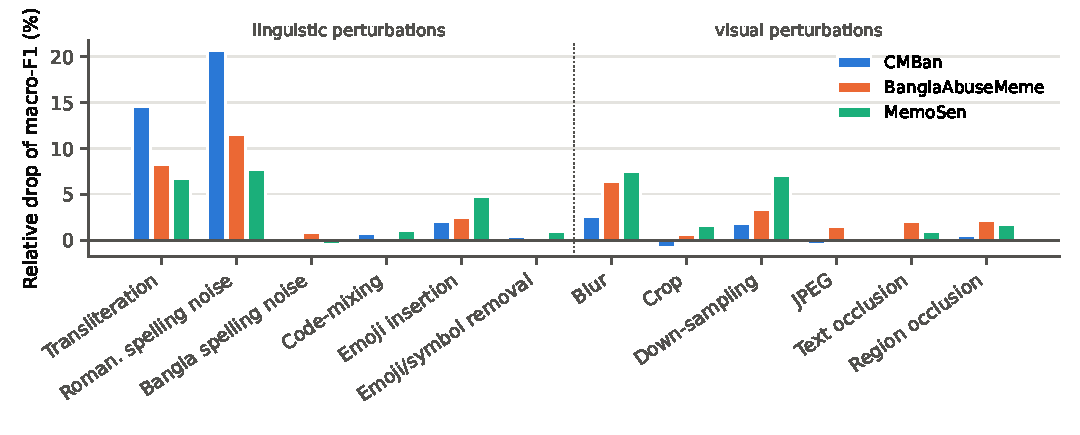
\includegraphics[width=\textwidth]{figures/cross_robustness.pdf}
  \caption{Relative Robustness Drop of the XLM-R + CLIP-B/32 fusion heads (mean over five heads, all tasks and three
  severities) for each perturbation family and dataset.}
  \label{fig:cross_rob}
\end{figure*}

\begin{table*}[t]
\centering
\small
\caption{Relative Robustness Drop (\%) across datasets, averaged over tasks and severities, for the matching unimodal heads (uni.) and the five XLM-R + CLIP-B/32 fusion heads (fus.; flip rate \% in parentheses). The top six rows are linguistic, the bottom six visual perturbations.}
\label{tab:cross_rob}
\begin{adjustbox}{max width=\textwidth}
\begin{tabular}{lcccccc}
\toprule
Perturbation & CMBan uni. & CMBan fus. & BAM uni. & BAM fus. & MemoSen uni. & MemoSen fus. \\
\midrule
Transliteration & 12.9 & 14.5 (37) & 18.4 & 8.2 (22) & 17.3 & 6.7 (21) \\
Roman. spelling noise & 17.9 & 20.7 (45) & 26.5 & 11.5 (28) & 21.8 & 7.7 (26) \\
Bangla spelling noise & 0.6 & 0.3 (7) & 1.7 & 0.8 (6) & 0.3 & -0.5 (8) \\
Code-mixing & -1.5 & 0.7 (8) & 0.7 & 0.3 (4) & 3.0 & 1.1 (8) \\
Emoji insertion & 2.3 & 2.0 (12) & 4.8 & 2.5 (11) & 11.7 & 4.8 (14) \\
Emoji/symbol removal & 1.0 & 0.4 (3) & 0.2 & 0.1 (1) & 3.5 & 0.9 (3) \\
Blur & 2.8 & 2.6 (23) & 16.6 & 6.3 (20) & 14.9 & 7.4 (27) \\
Crop & -1.9 & -0.7 (12) & 0.9 & 0.6 (10) & 3.3 & 1.6 (13) \\
Down-sampling & 2.2 & 1.9 (18) & 8.3 & 3.3 (15) & 13.4 & 7.1 (25) \\
JPEG & -0.0 & -0.5 (6) & 3.2 & 1.5 (8) & 0.8 & -0.1 (7) \\
Text occlusion & -0.3 & 0.3 (14) & 4.4 & 2.0 (11) & 4.0 & 1.0 (17) \\
Region occlusion & 1.4 & 0.5 (10) & 3.8 & 2.1 (11) & 4.5 & 1.6 (12) \\
\bottomrule
\end{tabular}
\end{adjustbox}
\end{table*}


Figure~\ref{fig:cross_rob} and Table~\ref{tab:cross_rob} summarise the Robustness Drop.
Figure~\ref{fig:sev_cmban} shows the CMBan severity curves.

\paragraph{Romanisation is the most damaging perturbation.} On every dataset, Romanised spelling noise is the
single most harmful perturbation for the fusion models. It costs 20.7\% (CMBan), 11.5\% (BAM) and 7.7\% (MemoSen) of
relative macro-F1 and changes 26--45\% of predictions. Transliteration without added noise costs 6.7--14.5\%. For the text-only heads, Romanised spelling noise costs
more still, at 17.9--26.5\%. By contrast, spelling noise in native Bangla script costs at most
1.7\%, and code-mixing at most 3\%. The damage is therefore caused by the \emph{change of script}, not by spelling
variation as such. A Romanised meme is tokenised by XLM-R into a different, and for Banglish poorly trained, part
of its vocabulary, so its embedding moves far from the Bangla-script training distribution.

\paragraph{Fusion mitigates text fragility only with enough data.} With sufficient training data, fusion halves the
damage of Romanisation relative to the text-only heads (BAM: 11.5 vs.\ 26.5\%; MemoSen: 7.7 vs.\ 21.8\%), because the
image branch keeps part of the decision intact. On CMBan the opposite happens. The fusion heads lose \emph{more}
than the text-only heads (20.7 vs.\ 17.9\%), and the Concat-MLP curve tracks the Text-MLP curve almost exactly
(Figure~\ref{fig:sev_cmban}). With 133 training memes, the fusion heads cannot learn to discount an unreliable
text input. Section~\ref{sec:results:xai} shows that, on all datasets, the perturbed text \emph{gains}
attribution share instead of losing it.

\paragraph{Visual robustness depends on how much the model uses the image.} Visual perturbations are almost harmless
on CMBan (at most 2.6\%), but on the larger datasets blur and down-sampling cost the image-only heads 8--17\% and
the fusion heads 3--7\%. On MemoSen, blur (7.4\%) is nearly as harmful as Romanisation (7.7\%). The difference
mirrors the benchmark: on the larger datasets the image models are more accurate and thus have more to lose.
Text-region occlusion, which removes up to all OCR regions from the image, costs only 0.3--2.0\% for fusion, and
JPEG compression and cropping cost the fusion heads at most 1.6\%.

\paragraph{Aggregate F1 hides instability.} Visual perturbations flip many predictions even when macro-F1 barely
moves. On CMBan, blur changes 23\% of fusion predictions at a 2.6\% F1 cost, because correct predictions that break
are offset by wrong predictions that become correct. Under severity-3 blur, 28\% of the memes that the fusion model
classifies correctly on Motivational become wrong. We therefore recommend reporting flip rates alongside Robustness
Drop.

\paragraph{Language groups.} Table~\ref{tab:cross_lang} breaks flip rates down by the script of the meme text.
\begin{itemize}
  \item Bangla-script memes flip most often under Romanisation (23--43\% for transliteration), because the
  perturbation rewrites all of their text.
  \item Code-mixed memes flip less (18--28\%), since part of their text is already in Latin script.
  \item Latin-script memes are, as a sanity check, almost unaffected by transliteration ($\leq$2.5\%). They still
  flip in 9--10\% of cases under spelling noise, which also affects English words.
\end{itemize}
Visual flip rates are similar across groups.

\begin{table}[t]
\centering
\small
\caption{Flip rate (\%) of the fusion heads by script/language group of the meme text.}
\label{tab:cross_lang}
\begin{adjustbox}{max width=\columnwidth}
\begin{tabular}{lcccccc}
\toprule
Dataset & Group & Transliteration & Roman. spelling noise & Code-mixing & Blur & Text occlusion \\
\midrule
CMBan & Bangla & 42.6 & 51.4 & 8.6 & 23.6 & 14.8 \\
CMBan & Code-mixed & 27.8 & 35.2 & 6.0 & 21.5 & 13.9 \\
BAM & Bangla & 23.2 & 29.8 & 4.5 & 20.1 & 10.9 \\
BAM & Code-mixed & 18.5 & 24.5 & 3.5 & 20.4 & 10.7 \\
BAM & Latin-script & 2.5 & 10.4 & 2.4 & 21.2 & 10.4 \\
MemoSen & Bangla & 25.4 & 29.6 & 8.5 & 28.5 & 16.9 \\
MemoSen & Code-mixed & 18.3 & 24.4 & 8.1 & 27.6 & 18.8 \\
MemoSen & Latin-script & 0.6 & 9.2 & 6.3 & 16.3 & 12.5 \\
\bottomrule
\end{tabular}
\end{adjustbox}
\end{table}


\begin{figure*}[t]
  \centering
  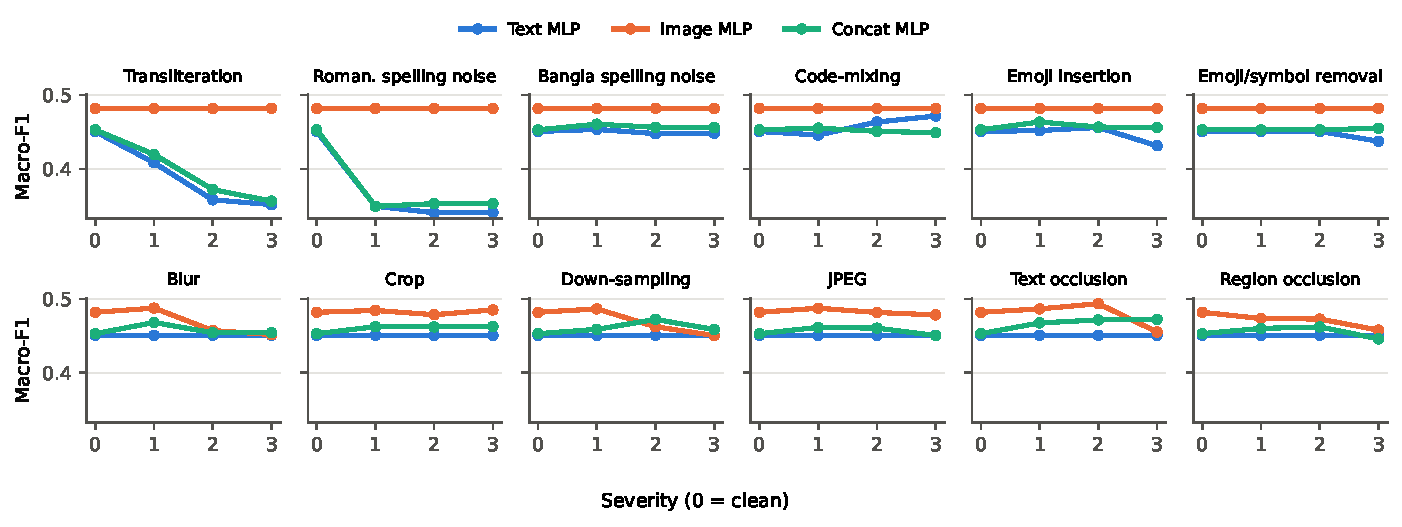
\includegraphics[width=\textwidth]{figures/cmban/severity_curves_coarse.pdf}
  \caption{CMBan: macro-F1 against perturbation severity for the text-only, image-only and Concat-MLP fusion heads
  (XLM-R + CLIP-B/32, coarse labels, mean over tasks).}
  \label{fig:sev_cmban}
\end{figure*}

% =====================================================================================
\subsection{Mitigation: Romanisation Augmentation}
\label{sec:results:aug}

\begin{table*}[t]
\centering
\small
\caption{Train-time Romanisation augmentation (XLM-R + CLIP-B/32). Macro-F1 (\%) on clean test folds and under transliteration and Romanised spelling noise (mean over heads, tasks and severities); relative Robustness Drop (\%) in parentheses. Spelling noise is unseen during training in the \emph{+translit.} setting.}
\label{tab:cross_aug}
\begin{adjustbox}{max width=\textwidth}
\begin{tabular}{lccccccc}
\toprule
Dataset & Augmentation & Text clean & Text translit. & Text noise & Fusion clean & Fusion translit. & Fusion noise \\
\midrule
CMBan & none & 45.5 & 39.7 (13) & 37.5 (18) & 47.2 & 40.6 (15) & 37.8 (21) \\
 & +translit. & 45.6 & 44.1 (3) & 43.2 (5) & 46.5 & 45.3 (2) & 44.0 (5) \\
 & +translit.\,+\,noise & 45.2 & 44.9 (1) & 45.7 (-1) & 46.1 & 46.2 (-1) & 46.0 (-0) \\
BAM & none & 59.2 & 48.2 (18) & 43.4 (26) & 65.0 & 59.8 (8) & 57.7 (12) \\
 & +translit. & 59.5 & 56.0 (6) & 53.7 (10) & 64.9 & 63.5 (2) & 63.1 (3) \\
 & +translit.\,+\,noise & 59.2 & 56.8 (4) & 55.5 (7) & 64.6 & 63.7 (2) & 63.4 (2) \\
MemoSen & none & 46.0 & 38.0 (17) & 36.0 (22) & 53.2 & 49.7 (7) & 49.1 (8) \\
 & +translit. & 45.5 & 43.2 (5) & 40.6 (11) & 53.6 & 52.4 (2) & 51.2 (4) \\
 & +translit.\,+\,noise & 45.2 & 43.7 (3) & 42.5 (6) & 53.5 & 52.7 (2) & 51.9 (3) \\
\bottomrule
\end{tabular}
\end{adjustbox}
\end{table*}


Table~\ref{tab:cross_aug} reports the augmentation experiment of Section~\ref{sec:method:aug}.

\paragraph{Transliteration augmentation removes most of the Romanisation drop.} Adding one transliterated copy of
each training meme reduces the relative drop of the fusion heads under transliteration from 15\% to 2\% on CMBan,
from 8\% to 2\% on BanglaAbuseMeme and from 7\% to 2\% on MemoSen. For the text-only heads, the reduction is from
13--18\% to 3--6\%.

\paragraph{It generalises to an unseen Romanisation style.} Romanised spelling noise is not used for augmentation in
this setting. Even so, the fusion drop under it falls from 21\% to 5\% (CMBan), 12\% to 3\% (BanglaAbuseMeme) and
8\% to 4\% (MemoSen). The heads thus learn to handle Romanised Bangla in general, not just the exact output of our
transliterator. Adding the noise style to training as well (\emph{+translit.\ + noise}) closes the remaining gap,
but only marginally improves on transliteration alone.

\paragraph{Clean accuracy is preserved.} The clean macro-F1 of the fusion heads changes by $-0.7$ (CMBan),
$-0.1$ (BanglaAbuseMeme) and $+0.4$ (MemoSen) points. The other linguistic perturbations are unaffected, apart
from changes of at most 1.3 points. Romanisation augmentation is therefore an almost free remedy for the main
weakness identified in Section~\ref{sec:results:rob}.

% =====================================================================================
\subsection{Explainability}
\label{sec:results:xai}

\begin{table*}[t]
\centering
\small
\caption{Explainability across datasets. Columns 2--8: text share of the Integrated-Gradients attribution of Concat-MLP on clean inputs and at severity 3. CAM ratio: Grad-CAM mass on OCR text boxes divided by their area share ($>1$: over-attention to rendered text). $r$: Pearson correlation of clean vs.\ perturbed CAMs (severity 2).}
\label{tab:cross_xai}
\begin{adjustbox}{max width=\textwidth}
\begin{tabular}{lcccccccccc}
\toprule
Dataset & Clean & Translit. & Roman. noise & Emoji ins. & Blur & Down-samp. & Text occ. & CAM ratio & $r$ blur & $r$ JPEG \\
\midrule
CMBan & 0.59 & 0.73 & 0.72 & 0.62 & 0.50 & 0.51 & 0.51 & 1.13 & 0.30 & 0.92 \\
BanglaAbuseMeme & 0.55 & 0.71 & 0.70 & 0.59 & 0.43 & 0.44 & 0.44 & 0.76 & 0.39 & 0.87 \\
MemoSen & 0.55 & 0.68 & 0.67 & 0.59 & 0.46 & 0.46 & 0.47 & 0.88 & 0.36 & 0.92 \\
\bottomrule
\end{tabular}
\end{adjustbox}
\end{table*}


\paragraph{Modality reliance.} On clean memes, the text embedding receives 55--59\% of the IG attribution of
Concat-MLP (Table~\ref{tab:cross_xai}, Figure~\ref{fig:share_cmban}). The perturbations shift this share in
opposite directions, and the pattern is the same on all three datasets.
\begin{itemize}
  \item \emph{Romanisation increases the text share} to 0.67--0.73. The perturbed text embedding lies far from the
  training mean that serves as the IG baseline, so it dominates the attribution. Instead of discounting an
  unfamiliar input, the head relies on it \emph{more}. This is the mechanism behind the large Romanisation drops.
  \item \emph{Visual degradation decreases the text share} to 0.43--0.51. Blur, down-sampling and text occlusion
  lower it by almost exactly the same amount. All three remove legible text from the image, which suggests that
  much of what the image branch adds to the decision is \emph{read} text that agrees with the text branch.
\end{itemize}

\begin{figure}[t]
  \centering
  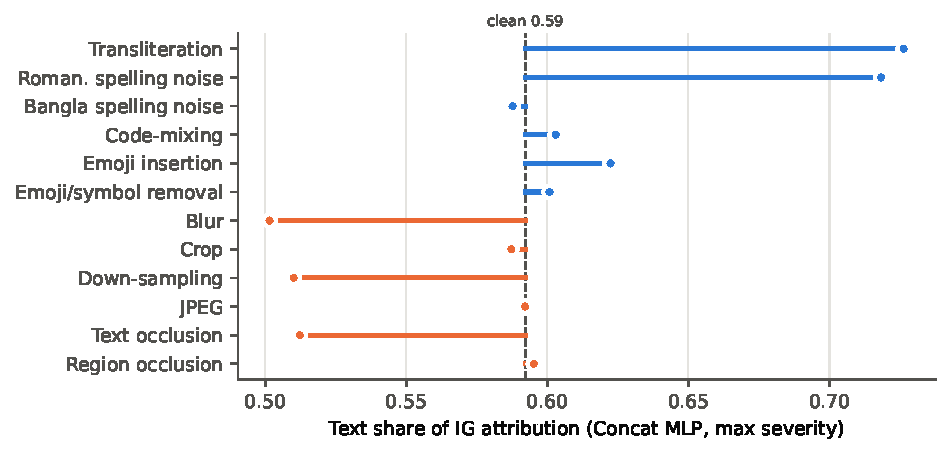
\includegraphics[width=\columnwidth]{figures/cmban/modality_share_shift.pdf}
  \caption{CMBan: shift of the text share of IG attribution (Concat-MLP) from clean inputs (dashed line) to
  severity-3 perturbations. Blue: linguistic, orange: visual. BAM and MemoSen show the same pattern
  (Table~\ref{tab:cross_xai}).}
  \label{fig:share_cmban}
\end{figure}

\paragraph{Visual attention.} The Grad-CAM text-attention ratio of CLIP-B/32 differs between datasets.
\begin{itemize}
  \item On CMBan it is 1.13: CLIP over-attends to the rendered caption, consistent with its known ability to read
  text.
  \item On BAM (0.76) and MemoSen (0.88), the captions receive \emph{less} attention than their area would warrant.
\end{itemize}
CMBan memes are cartoon panels with large speech bubbles, while many BAM and MemoSen memes are photographs with a
short caption band, where faces and scenes compete for attention. The claim that CLIP mainly attends to text
therefore does not generalise beyond cartoon memes.

The stability of the maps is consistent across datasets:
\begin{itemize}
  \item The maps are stable under JPEG compression ($r=0.87$--$0.92$).
  \item They are unstable under blur ($r=0.30$--$0.39$) and down-sampling ($r\approx0.5$--$0.6$), even when the
  prediction is unchanged.
\end{itemize}
Figure~\ref{fig:gradcam_cmban} shows CMBan examples. After text occlusion, the attention moves to the remaining text
and to the cartoon characters. The letterbox padding also attracts attention, which suggests that it should be
masked in future work.

\begin{figure*}[t]
  \centering
  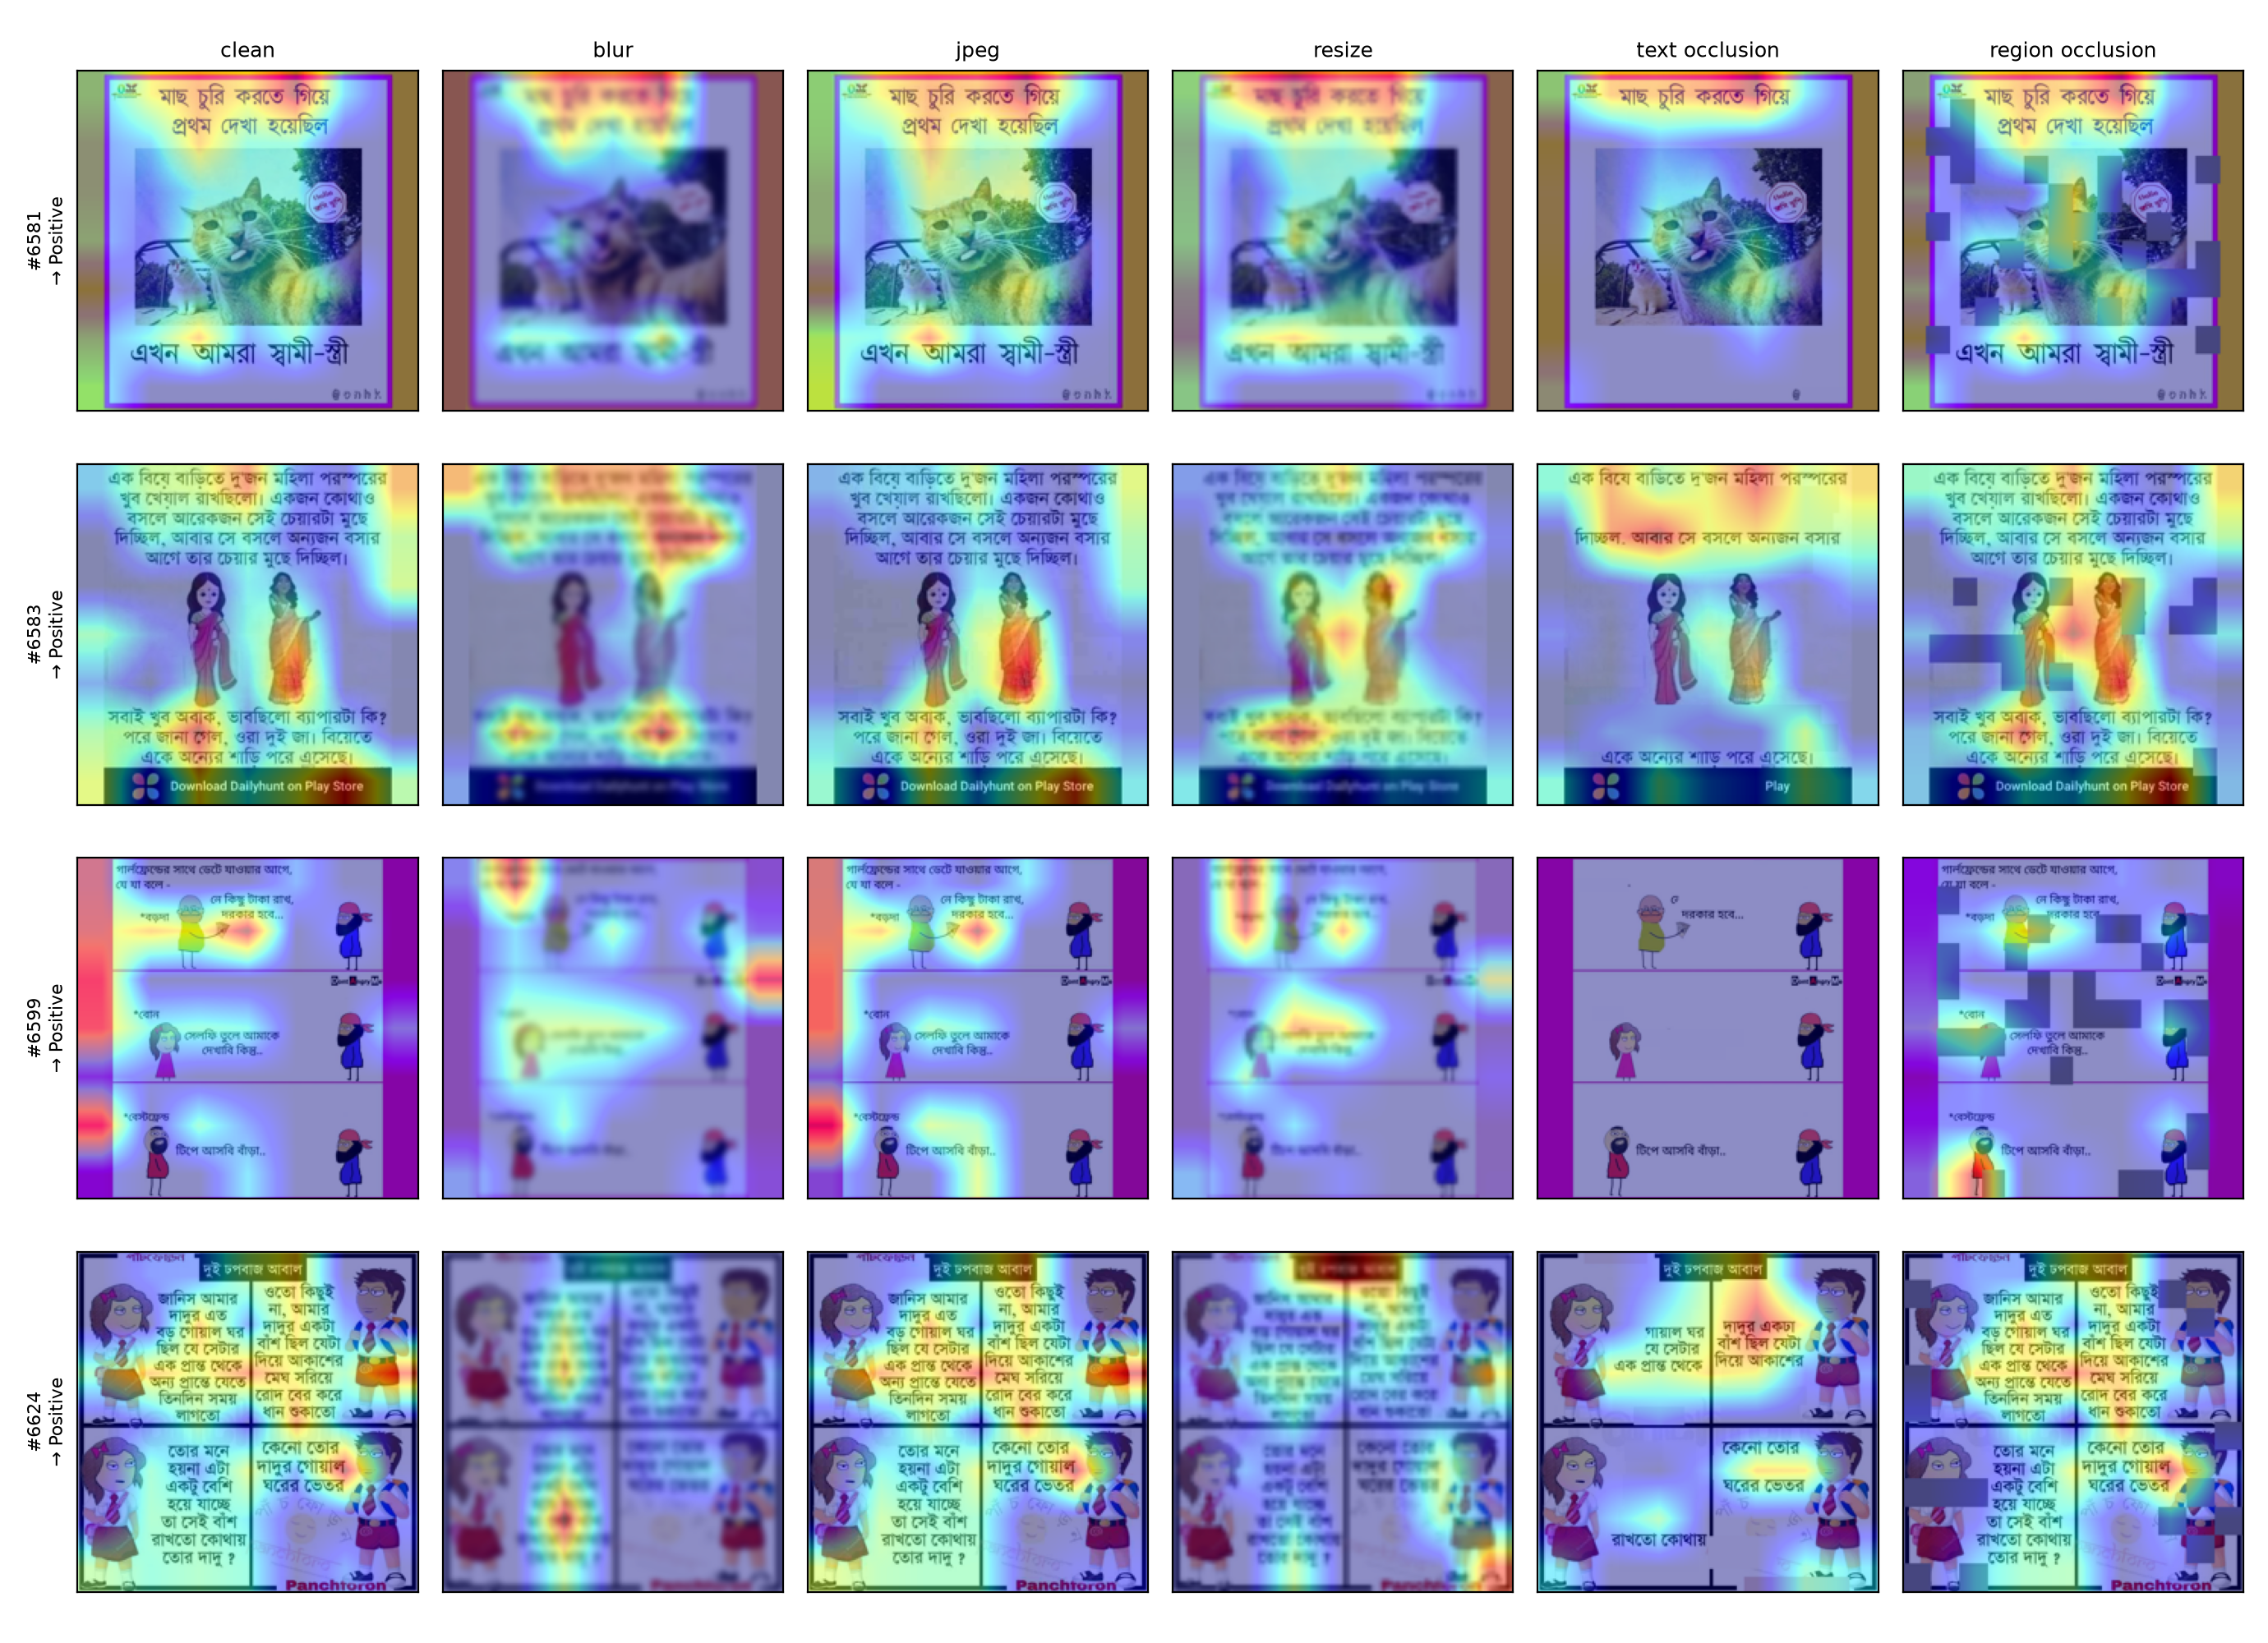
\includegraphics[width=0.85\textwidth]{figures/cmban/gradcam_examples.png}
  \caption{CMBan: Grad-CAM on CLIP ViT-B/32 (sentiment head) for four memes under the spatially aligned visual
  perturbations at severity 2.}
  \label{fig:gradcam_cmban}
\end{figure*}

% =====================================================================================
\subsection{Error Analysis}
\label{sec:results:errors}

\begin{table*}[t]
\centering
\small
\caption{Clean-data error categories of the primary fusion model (\% of memes, averaged over tasks).}
\label{tab:cross_err}
\begin{adjustbox}{max width=\textwidth}
\begin{tabular}{lcccccc}
\toprule
Dataset & Contextual/cultural & Correct & Cross modal & Linguistic & OCR limited & Visual \\
\midrule
CMBan & 17.6 & 55.2 & 3.6 & 8.7 & 6.0 & 8.9 \\
BanglaAbuseMeme & 10.8 & 67.8 & 0.9 & 7.3 & 6.8 & 6.3 \\
MemoSen & 10.4 & 68.5 & 3.2 & 5.7 & 6.3 & 5.8 \\
\bottomrule
\end{tabular}
\end{adjustbox}
\end{table*}

\begin{table}[t]
\centering
\small
\caption{Robustness fragility categories (\% of memes, averaged over tasks; severity $\geq 2$).}
\label{tab:cross_frag}
\begin{adjustbox}{max width=\columnwidth}
\begin{tabular}{lccccc}
\toprule
Dataset & Clean error & Cross modal fragile & Linguistic fragile & Stable & Visual fragile \\
\midrule
CMBan & 43.3 & 20.5 & 18.5 & 11.1 & 6.6 \\
BanglaAbuseMeme & 32.2 & 13.6 & 11.1 & 32.7 & 10.5 \\
MemoSen & 31.2 & 19.3 & 14.7 & 22.2 & 12.7 \\
\bottomrule
\end{tabular}
\end{adjustbox}
\end{table}


\paragraph{Clean errors.} Table~\ref{tab:cross_err} attributes the clean errors of the best learned XLM-R +
CLIP-B/32 fusion head. Late fusion is excluded, because it averages the two unimodal models and cannot, for binary
tasks, fail when both are right.
\begin{itemize}
  \item The largest error category on every dataset is \emph{contextual/cultural}: 18\% of CMBan memes and 10--11\%
  of BAM and MemoSen memes. Here all three models fail although readable text is available.
  \item The category peaks on Sentiment (27\% on CMBan, 18\% on BAM) and on CMBan Sarcasm and Humour (20\%).
  \item The memes in this category typically depend on knowledge outside the meme, such as a film, a public figure
  or a template whose meaning has drifted.
\end{itemize}
Linguistic and visual errors are about equally common (6--9\% each), and OCR-limited errors account for 6--7\%.
\emph{Cross-modal} errors, where both unimodal models are right but fusion is wrong, are rare (1--4\%). The learned
fusion heads seldom destroy information that either modality has, but they also rarely recover memes that both
modalities miss.

\paragraph{Fragility.} Table~\ref{tab:cross_frag} classifies each meme by its behaviour under perturbations of
severity $\geq2$.
\begin{itemize}
  \item Only 11\% (CMBan) to 33\% (BAM) of memes are \emph{stable}: correct on clean data and under every
  perturbation.
  \item Among the memes that are correct on clean data, cross-modal fragility (broken by both a linguistic and a
  visual perturbation) is the most common failure type on all three datasets (13.6--20.5\% of all memes).
  \item On CMBan, linguistic fragility dominates the Offensive task (44\%). Offensive memes are often recognised from
  a few Bangla swear words, which Romanisation disguises.
\end{itemize}
